% ============================================================
%  L01_mini10.tex  --  Fintech Foundations and Overview
%  MINI-10 variant: 10 slides, self-contained, inline TikZ/pgfplots only
%  Variant 5 per fintech-lecture-01.md Part 2
% ============================================================
\documentclass[aspectratio=169, 11pt]{beamer}
\usetheme{Madrid}
\usecolortheme{whale}
\usepackage{tikz,pgfplots,booktabs,multicol,amsmath}
\usetikzlibrary{arrows.meta,positioning,shapes.geometric,calc,decorations.pathmorphing}
\pgfplotsset{compat=1.18}

% ---- Colour palette ----------------------------------------
\definecolor{mlpurple}{HTML}{9467BD}
\definecolor{mlblue}{HTML}{1F77B4}
\definecolor{mlred}{HTML}{D62728}
\definecolor{mlorange}{HTML}{FF7F0E}
\definecolor{mlgreen}{HTML}{2CA02C}
\definecolor{mlgray}{HTML}{7F7F7F}
\definecolor{mlteal}{HTML}{0D7377}
\definecolor{mlcyan}{HTML}{14BDEB}

% ---- Beamer theme overrides --------------------------------
\setbeamercolor{structure}{fg=mlteal}
\setbeamercolor{palette primary}{bg=mlteal,fg=white}
\setbeamercolor{palette secondary}{bg=mlteal!80,fg=white}
\setbeamercolor{palette tertiary}{bg=mlteal!60,fg=white}
\setbeamercolor{palette quaternary}{bg=mlteal,fg=white}
\setbeamercolor{frametitle}{bg=mlteal!10,fg=mlteal}
\setbeamercolor{title}{fg=white}
\setbeamercolor{subtitle}{fg=mlcyan}
\setbeamercolor{block title}{bg=mlteal,fg=white}
\setbeamercolor{block body}{bg=mlteal!8,fg=black}
\setbeamercolor{block title alerted}{bg=mlred,fg=white}
\setbeamercolor{block body alerted}{bg=mlred!8,fg=black}
\setbeamercolor{block title example}{bg=mlgreen,fg=white}
\setbeamercolor{block body example}{bg=mlgreen!8,fg=black}
\setbeamerfont{frametitle}{size=\large,series=\bfseries}

% ---- Bottom note command -----------------------------------
\newcommand{\bottomnote}[1]{%
  \vfill
  \begin{beamercolorbox}[wd=\textwidth,ht=2ex,dp=1ex]{palette primary}
    \tiny\hspace{1em}#1
  \end{beamercolorbox}}

% ---- Metadata ----------------------------------------------
\title{Fintech Foundations and Overview}
\subtitle{10-Slide Mini Lecture}
\author{Joerg Osterrieder}
\institute{University of Zurich}
\date{Spring 2026}
\setbeamertemplate{navigation symbols}{}

% ============================================================
\begin{document}
% ============================================================

% ============================================================
%  FRAME 1 -- WHY: TikZ comic (banker vs fintech founder)
% ============================================================
\begin{frame}{Why This Matters: Two Worlds Collide}
\begin{center}
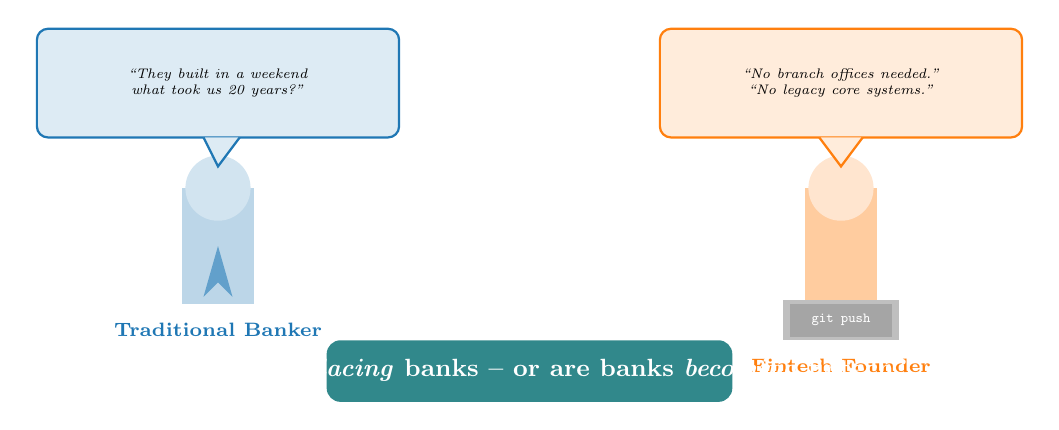
\begin{tikzpicture}[scale=0.92]

  % ---- Banker figure (left) ----------------------------------
  % body
  \fill[mlblue!30] (-4.8,0) rectangle (-3.8,1.6);
  % head
  \fill[mlblue!20] (-4.3,1.6) circle (0.45);
  % tie
  \fill[mlblue!70] (-4.3,0.8) -- (-4.5,0.1) -- (-4.3,0.3) -- (-4.1,0.1) -- cycle;
  % label
  \node[font=\scriptsize\bfseries,text=mlblue] at (-4.3,-0.35) {Traditional Banker};

  % Banker speech bubble
  \fill[mlblue!15,rounded corners=4pt]
    (-6.8,2.3) rectangle (-1.8,3.8);
  \draw[mlblue,thick,rounded corners=4pt]
    (-6.8,2.3) rectangle (-1.8,3.8);
  % bubble tail
  \fill[mlblue!15] (-4.5,2.3) -- (-4.3,1.9) -- (-4.0,2.3) -- cycle;
  \draw[mlblue,thick] (-4.5,2.3) -- (-4.3,1.9) -- (-4.0,2.3);
  \node[font=\tiny,text width=4.6cm,align=center] at (-4.3,3.05)
    {\textit{``They built in a weekend}\\\textit{what took us 20 years?"}};

  % ---- Fintech founder figure (right) ------------------------
  % body (casual)
  \fill[mlorange!40] (3.8,0) rectangle (4.8,1.6);
  % head
  \fill[mlorange!20] (4.3,1.6) circle (0.45);
  % laptop
  \fill[mlgray!50] (3.5,-0.5) rectangle (5.1,0.05);
  \fill[mlgray!70] (3.6,-0.45) rectangle (5.0,0.0);
  \node[font=\tiny,text=white] at (4.3,-0.22) {\texttt{git push}};
  % label
  \node[font=\scriptsize\bfseries,text=mlorange] at (4.3,-0.85) {Fintech Founder};

  % Founder speech bubble
  \fill[mlorange!15,rounded corners=4pt]
    (1.8,2.3) rectangle (6.8,3.8);
  \draw[mlorange,thick,rounded corners=4pt]
    (1.8,2.3) rectangle (6.8,3.8);
  % bubble tail
  \fill[mlorange!15] (4.0,2.3) -- (4.3,1.9) -- (4.6,2.3) -- cycle;
  \draw[mlorange,thick] (4.0,2.3) -- (4.3,1.9) -- (4.6,2.3);
  \node[font=\tiny,text width=4.6cm,align=center] at (4.3,3.05)
    {\textit{``No branch offices needed."}\\\textit{``No legacy core systems."}};

  % ---- Central tension banner --------------------------------
  \fill[mlteal!85,rounded corners=5pt] (-2.8,-1.35) rectangle (2.8,-0.5);
  \node[font=\small\bfseries,text=white,align=center] at (0,-0.92)
    {Is fintech \emph{replacing} banks -- or are banks \emph{becoming} fintech?};

\end{tikzpicture}
\end{center}
\bottomnote{Core tension: Technology is reshaping finance faster than any force since the printing press.}
\end{frame}

% ============================================================
%  FRAME 2 -- FEEL: Text-only prompt (phone app exercise)
% ============================================================
\begin{frame}{The Fintech in Your Pocket}

\vspace{0.4em}
\begin{block}{A 90-Second Personal Audit}
Think about the last 48 hours.  How many financial transactions did you make?\\[0.4em]
How many involved a \textbf{traditional bank branch}?
\end{block}

\vspace{0.6em}
Now open your phone.  Count the apps that \emph{touch your money}:

\vspace{0.4em}
\begin{columns}[T]
\begin{column}{0.48\textwidth}
\begin{itemize}
  \item[\textcolor{mlteal}{\textbullet}] \textbf{Banking} -- current account, savings
  \item[\textcolor{mlteal}{\textbullet}] \textbf{Payments} -- contactless, P2P, wallets
  \item[\textcolor{mlteal}{\textbullet}] \textbf{Investment} -- robo-advisor, brokerage
\end{itemize}
\end{column}
\begin{column}{0.48\textwidth}
\begin{itemize}
  \item[\textcolor{mlcyan}{\textbullet}] \textbf{Insurance} -- on-demand, auto, health
  \item[\textcolor{mlcyan}{\textbullet}] \textbf{Lending} -- BNPL, credit line, mortgage
  \item[\textcolor{mlcyan}{\textbullet}] \textbf{Budgeting} -- spending analytics, alerts
\end{itemize}
\end{column}
\end{columns}

\vspace{0.7em}
\begin{exampleblock}{Quick Exercise -- Bring Your Count to the Discussion}
For each app: is it from a \textbf{traditional bank}, a \textbf{fintech startup}, or a \textbf{big tech company}?\\
Typical MSc student: \textbf{5--10 financial apps} -- and most are \emph{not} from their bank.
\end{exampleblock}

\bottomnote{This exercise recurs in L02 (Fintech Ecosystem). The pattern you notice today will deepen throughout the course.}
\end{frame}

% ============================================================
%  FRAME 3 -- WHAT: Comparison table (bank vs fintech, 5 dimensions)
% ============================================================
\begin{frame}{Traditional Bank vs.\ Fintech: Five Dimensions}

\vspace{0.3em}
\begin{center}
\small
\begin{tabular}{@{}lll@{}}
\toprule
\textbf{Dimension} & \textbf{Traditional Bank} & \textbf{Fintech Startup} \\
\midrule
\textbf{Speed to market}
  & Months to years (legacy IT, sign-off cycles)
  & Days to weeks (agile, cloud-native) \\[4pt]
\textbf{Cost structure}
  & High fixed costs (branches, compliance staff)
  & Low marginal cost (software scales freely) \\[4pt]
\textbf{Customer experience}
  & Consistent but often friction-heavy
  & Mobile-first, instant, highly personalised \\[4pt]
\textbf{Regulatory position}
  & Fully licensed, supervised, deposit-insured
  & Often operating under exemptions or gaps \\[4pt]
\textbf{Trust \& resilience}
  & Deep institutional trust, proven resilience
  & Trust must be earned; failure rate is high \\
\bottomrule
\end{tabular}
\end{center}

\vspace{0.5em}
\begin{block}{The Strategic Insight}
Neither side holds all the advantages.  The most powerful fintech products
\emph{combine} bank-grade trust and licence with fintech-grade speed and experience.
\end{block}

\bottomnote{The \textit{unbundling thesis}: fintech companies attack the most profitable or least efficient slice of each dimension.}
\end{frame}

% ============================================================
%  FRAME 4 -- CASE: Step diagram (2008 crisis causal chain)
% ============================================================
\begin{frame}{The 2008 Crisis: A Catalyst, Not a Cause}
\vspace{0.2em}
\begin{center}
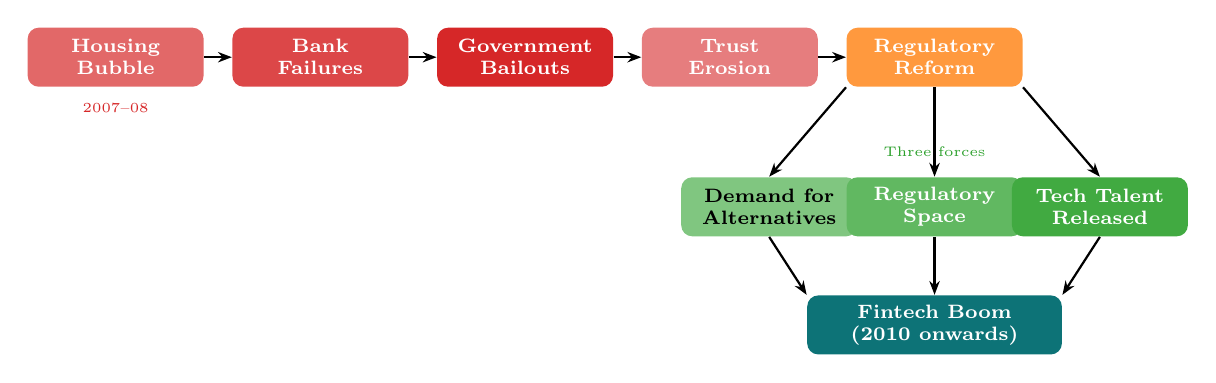
\begin{tikzpicture}[
  box/.style={rectangle,rounded corners=4pt,minimum width=2.0cm,
              minimum height=0.75cm,font=\scriptsize\bfseries,
              text centered,text width=2.0cm},
  arr/.style={-{Stealth[length=5pt]},thick}
]

% Row 1: causal chain (left to right)
\node[box,fill=mlred!70,text=white]       (hb)  at (0,0)    {Housing\\Bubble};
\node[box,fill=mlred!85,text=white]       (bf)  at (2.6,0)  {Bank\\Failures};
\node[box,fill=mlred,text=white]          (ba)  at (5.2,0)  {Government\\Bailouts};
\node[box,fill=mlred!60,text=white]       (te)  at (7.8,0)  {Trust\\Erosion};
\node[box,fill=mlorange!80,text=white]    (rr)  at (10.4,0) {Regulatory\\Reform};

\draw[arr] (hb) -- (bf);
\draw[arr] (bf) -- (ba);
\draw[arr] (ba) -- (te);
\draw[arr] (te) -- (rr);

% Row 2: three outputs from regulatory reform (fan out downward)
\node[box,fill=mlgreen!60,text=black]     (d1) at (8.3,-1.9)  {Demand for\\Alternatives};
\node[box,fill=mlgreen!75,text=white]     (d2) at (10.4,-1.9) {Regulatory\\Space};
\node[box,fill=mlgreen!90,text=white]     (d3) at (12.5,-1.9) {Tech Talent\\Released};

\draw[arr] (rr.south west) -- (d1.north);
\draw[arr] (rr.south)      -- (d2.north);
\draw[arr] (rr.south east) -- (d3.north);

% Final outcome
\node[box,fill=mlteal,text=white,minimum width=3.2cm,text width=3.0cm]
      (fin) at (10.4,-3.4) {Fintech Boom\\(2010 onwards)};

\draw[arr] (d1.south) -- (fin.north west);
\draw[arr] (d2.south) -- (fin.north);
\draw[arr] (d3.south) -- (fin.north east);

% Year annotation
\node[font=\tiny,text=mlred] at (0,-0.65) {2007--08};
\node[font=\tiny,text=mlgreen] at (10.4,-1.2) {Three forces};

\end{tikzpicture}
\end{center}
\vspace{0.1em}
\begin{block}{}
\scriptsize The crisis did \textbf{not} cause fintech -- it removed the barriers
(trust, regulation, talent) that had held fintech back for a decade.
\end{block}
\bottomnote{By 2010, consumer trust in banks had fallen to historic lows in the US, UK, and Eurozone -- creating demand for alternatives.}
\end{frame}

% ============================================================
%  FRAME 5 -- HOW: Architecture diagram (4 collaboration models)
% ============================================================
\begin{frame}{How Banks and Fintechs Work Together: Four Models}
\vspace{0.15em}
\begin{center}
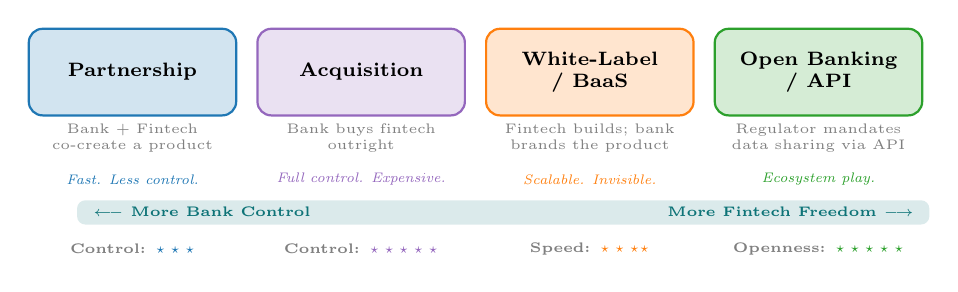
\begin{tikzpicture}[scale=0.88,
  modbox/.style={rectangle,rounded corners=5pt,minimum width=2.6cm,
                 minimum height=1.1cm,font=\scriptsize\bfseries,
                 text centered,text width=2.4cm},
  attrib/.style={font=\tiny,text=mlgray,text width=2.3cm,align=center}
]

% ---- Model 1: Partnership -----------------------------------
\node[modbox,fill=mlblue!20,draw=mlblue,thick]   (p1) at (0,0)    {Partnership};
\node[attrib] at (0,-0.95) {Bank + Fintech\\co-create a product};
\node[font=\tiny\itshape,text=mlblue] at (0,-1.55) {Fast. Less control.};

% ---- Model 2: Acquisition ----------------------------------
\node[modbox,fill=mlpurple!20,draw=mlpurple,thick] (p2) at (3.3,0) {Acquisition};
\node[attrib] at (3.3,-0.95) {Bank buys fintech\\outright};
\node[font=\tiny\itshape,text=mlpurple] at (3.3,-1.55) {Full control. Expensive.};

% ---- Model 3: White-Label / BaaS ---------------------------
\node[modbox,fill=mlorange!20,draw=mlorange,thick] (p3) at (6.6,0) {White-Label\\/ BaaS};
\node[attrib] at (6.6,-0.95) {Fintech builds; bank\\brands the product};
\node[font=\tiny\itshape,text=mlorange] at (6.6,-1.55) {Scalable. Invisible.};

% ---- Model 4: Open Banking / API ---------------------------
\node[modbox,fill=mlgreen!20,draw=mlgreen,thick]   (p4) at (9.9,0) {Open Banking\\/ API};
\node[attrib] at (9.9,-0.95) {Regulator mandates\\data sharing via API};
\node[font=\tiny\itshape,text=mlgreen] at (9.9,-1.55) {Ecosystem play.};

% ---- Spectrum bar ------------------------------------------
\fill[mlteal!15,rounded corners=3pt] (-0.8,-2.2) rectangle (11.5,-1.85);
\node[font=\tiny\bfseries,text=mlteal] at (1.0,-2.02) {$\longleftarrow$ More Bank Control};
\node[font=\tiny\bfseries,text=mlteal] at (9.5,-2.02) {More Fintech Freedom $\longrightarrow$};

% ---- Scoring table (compact) --------------------------------
\node[font=\tiny\bfseries,text=mlgray] at (0,-2.55)    {Control: \textcolor{mlblue}{$\star\star\star$}};
\node[font=\tiny\bfseries,text=mlgray] at (3.3,-2.55)  {Control: \textcolor{mlpurple}{$\star\star\star\star\star$}};
\node[font=\tiny\bfseries,text=mlgray] at (6.6,-2.55)  {Speed: \textcolor{mlorange}{$\star\star\star\star$}};
\node[font=\tiny\bfseries,text=mlgray] at (9.9,-2.55)  {Openness: \textcolor{mlgreen}{$\star\star\star\star\star$}};

\end{tikzpicture}
\end{center}
\vspace{0.05em}
\begin{block}{}
\scriptsize Most large banks use \textbf{multiple models simultaneously} -- partnering in payments,
acquiring in lending, white-labelling for compliance infrastructure.
\end{block}
\bottomnote{PSD2 (EU 2018) made open banking mandatory, turning the bank's data moat into a shared resource for all authorised third parties.}
\end{frame}

% ============================================================
%  FRAME 6 -- RISK: TikZ comic (fintech failure scene)
% ============================================================
\begin{frame}{When Fintech Fails: Four Failure Modes}
\begin{columns}[T]
\begin{column}{0.48\textwidth}
\vspace{0.3em}
\begin{center}
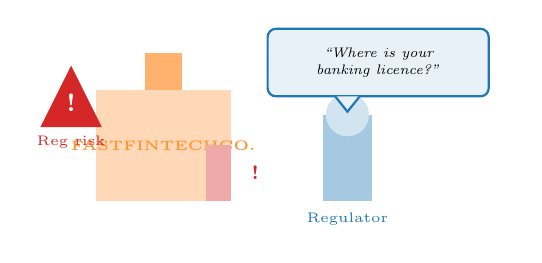
\begin{tikzpicture}[scale=0.78]

  % Fintech startup building (simple icon)
  \fill[mlorange!30] (-1.1,0) rectangle (1.1,1.8);
  \fill[mlorange!60] (-0.3,1.8) rectangle (0.3,2.4); % roof peak
  \node[font=\tiny\bfseries,text=mlorange!80] at (0,0.9) {FAST\\FINTECH\\CO.};

  % Crumbling corner
  \fill[mlred!40] (0.7,0) rectangle (1.1,0.9);
  \node[font=\scriptsize,text=mlred] at (1.5,0.45) {\textbf{!}};

  % Regulator figure
  \fill[mlblue!40] (2.6,0) rectangle (3.4,1.4);
  \fill[mlblue!20] (3.0,1.4) circle (0.35);
  \node[font=\tiny,text=mlblue] at (3.0,-0.3) {Regulator};

  % Speech bubble from regulator
  \fill[mlblue!10,rounded corners=3pt] (1.7,1.7) rectangle (5.3,2.8);
  \draw[mlblue,thick,rounded corners=3pt] (1.7,1.7) rectangle (5.3,2.8);
  \fill[mlblue!10] (2.8,1.7) -- (3.0,1.45) -- (3.2,1.7) -- cycle;
  \draw[mlblue,thick] (2.8,1.7) -- (3.0,1.45) -- (3.2,1.7);
  \node[font=\tiny,text width=3.2cm,align=center] at (3.5,2.25)
    {\textit{``Where is your\\banking licence?"}};

  % Warning sign
  \fill[mlred] (-2.0,1.2) -- (-1.5,2.2) -- (-1.0,1.2) -- cycle;
  \node[font=\small\bfseries,text=white] at (-1.5,1.6) {!};
  \node[font=\tiny,text=mlred] at (-1.5,0.95) {Reg risk};

\end{tikzpicture}
\end{center}
\end{column}
\begin{column}{0.48\textwidth}
\vspace{0.5em}
\begin{alertblock}{Failure Mode 1 -- Regulatory Risk}
\tiny Operating without adequate licences; crossing jurisdictional lines undetected until enforcement.
\end{alertblock}
\vspace{0.25em}
\begin{alertblock}{Failure Mode 2 -- Trust Risk}
\tiny Data breaches; no deposit insurance; opaque complaint resolution erode user confidence overnight.
\end{alertblock}
\vspace{0.25em}
\begin{alertblock}{Failure Mode 3 -- Unit Economics}
\tiny Customer acquisition cost exceeds lifetime value; free accounts attract cost-conscious users who never generate revenue.
\end{alertblock}
\vspace{0.25em}
\begin{alertblock}{Failure Mode 4 -- Systemic Risk}
\tiny Concentration in single cloud providers; API interdependence creates new ``too-connected-to-fail'' dynamics.
\end{alertblock}
\end{column}
\end{columns}
\bottomnote{Fintech disruption is not risk-free. The question is whether fintech creates new risks -- or merely redistributes existing ones to less protected parties.}
\end{frame}

% ============================================================
%  FRAME 7 -- WHERE: pgfplots bar chart (regional adoption)
% ============================================================
\begin{frame}{Where Is Fintech Winning? Regional Adoption Patterns}
\vspace{0.1em}
\begin{center}
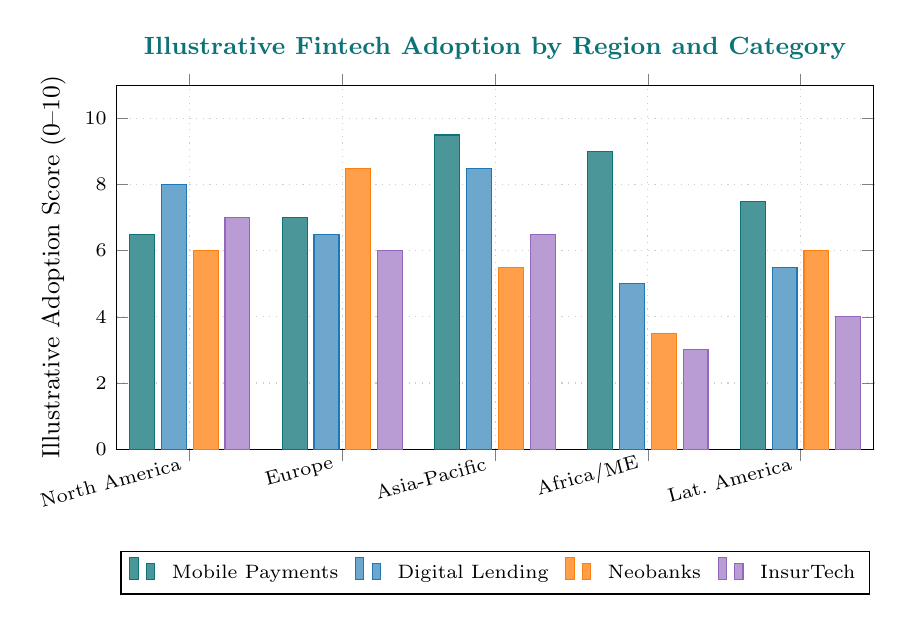
\begin{tikzpicture}
\begin{axis}[
  width=11.2cm, height=6.2cm,
  ybar=2.5pt,
  bar width=9pt,
  enlarge x limits=0.12,
  ylabel={\small Illustrative Adoption Score (0--10)},
  ylabel style={font=\small},
  symbolic x coords={North America, Europe, Asia-Pacific, Africa/ME, Lat.\ America},
  xtick=data,
  xticklabel style={font=\scriptsize, rotate=15, anchor=east},
  ymin=0, ymax=11,
  ytick={0,2,4,6,8,10},
  yticklabel style={font=\scriptsize},
  legend style={font=\scriptsize, at={(0.5,-0.28)}, anchor=north,
                legend columns=4, column sep=4pt},
  legend cell align=left,
  grid=major,
  grid style={dotted,mlgray!40},
  title={\small\bfseries\textcolor{mlteal}{Illustrative Fintech Adoption by Region and Category}},
  title style={font=\small},
  clip=false,
]
% Mobile Payments
\addplot[fill=mlteal!75,draw=mlteal] coordinates {
  (North America,6.5) (Europe,7.0) (Asia-Pacific,9.5)
  (Africa/ME,9.0) (Lat.\ America,7.5)};
% Digital Lending
\addplot[fill=mlblue!65,draw=mlblue] coordinates {
  (North America,8.0) (Europe,6.5) (Asia-Pacific,8.5)
  (Africa/ME,5.0) (Lat.\ America,5.5)};
% Neobanks
\addplot[fill=mlorange!75,draw=mlorange] coordinates {
  (North America,6.0) (Europe,8.5) (Asia-Pacific,5.5)
  (Africa/ME,3.5) (Lat.\ America,6.0)};
% InsurTech
\addplot[fill=mlpurple!65,draw=mlpurple] coordinates {
  (North America,7.0) (Europe,6.0) (Asia-Pacific,6.5)
  (Africa/ME,3.0) (Lat.\ America,4.0)};

\legend{Mobile Payments, Digital Lending, Neobanks, InsurTech}
\end{axis}
\end{tikzpicture}
\end{center}
\vspace{-0.3em}
{\tiny\textcolor{mlgray}{Conceptual adoption levels -- illustrative comparison only.
Asia-Pacific leads in mobile payments; Europe in neobanks; North America in digital lending.}}
\bottomnote{The ``leapfrog effect'': regions with weak traditional banking infrastructure often adopt fintech faster (M-Pesa, Alipay, PIX are non-Western innovations).}
\end{frame}

% ============================================================
%  FRAME 8 -- IMPACT: Stakeholder map (winners/losers)
% ============================================================
\begin{frame}{Who Wins, Who Loses? A Stakeholder Map}
\vspace{0.2em}
\begin{center}
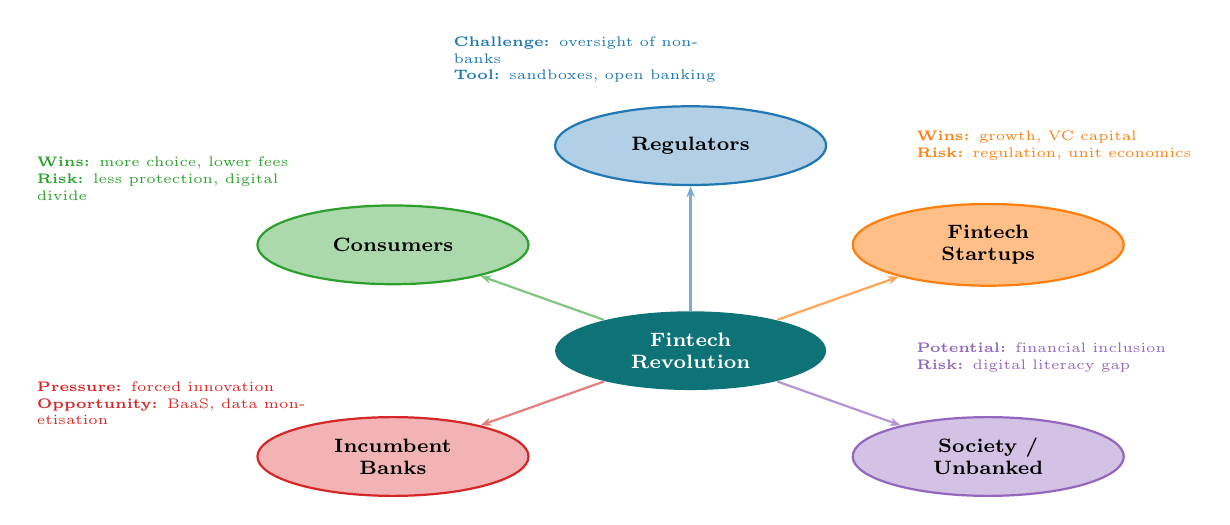
\begin{tikzpicture}[scale=0.84,
  stk/.style={ellipse,minimum width=2.4cm,minimum height=1.0cm,
              font=\scriptsize\bfseries,text centered,text width=2.2cm},
  lbl/.style={font=\tiny,text width=3.5cm,align=left}
]

% Central node
\node[stk,fill=mlteal,text=white,minimum width=2.8cm]
  (ctr) at (0,0) {Fintech\\Revolution};

% ---- Stakeholder nodes (radial) ----------------------------
\node[stk,fill=mlgreen!40,draw=mlgreen,thick]
  (con) at (-4.5, 1.6) {Consumers};
\node[stk,fill=mlred!35,draw=mlred,thick]
  (bnk) at (-4.5,-1.6) {Incumbent\\Banks};
\node[stk,fill=mlblue!35,draw=mlblue,thick]
  (reg) at (0, 3.1)   {Regulators};
\node[stk,fill=mlorange!50,draw=mlorange,thick]
  (ftc) at (4.5, 1.6)  {Fintech\\Startups};
\node[stk,fill=mlpurple!40,draw=mlpurple,thick]
  (soc) at (4.5,-1.6)  {Society /\\Unbanked};

% ---- Edges -------------------------------------------------
\draw[mlgreen!60,thick,-{Stealth[length=4pt]}] (ctr) -- (con);
\draw[mlred!60,thick,-{Stealth[length=4pt]}]   (ctr) -- (bnk);
\draw[mlblue!60,thick,-{Stealth[length=4pt]}]  (ctr) -- (reg);
\draw[mlorange!70,thick,-{Stealth[length=4pt]}](ctr) -- (ftc);
\draw[mlpurple!70,thick,-{Stealth[length=4pt]}](ctr) -- (soc);

% ---- Outcome labels ----------------------------------------
\node[lbl,text=mlgreen] at (-7.8, 2.6)
  {\textbf{Wins:} more choice, lower fees\\
   \textbf{Risk:} less protection, digital divide};
\node[lbl,text=mlred] at (-7.8,-0.8)
  {\textbf{Pressure:} forced innovation\\
   \textbf{Opportunity:} BaaS, data monetisation};
\node[lbl,text=mlblue] at (-1.5, 4.4)
  {\textbf{Challenge:} oversight of non-banks\\
   \textbf{Tool:} sandboxes, open banking};
\node[lbl,text=mlorange] at (5.5, 3.1)
  {\textbf{Wins:} growth, VC capital\\
   \textbf{Risk:} regulation, unit economics};
\node[lbl,text=mlpurple] at (5.5,-0.1)
  {\textbf{Potential:} financial inclusion\\
   \textbf{Risk:} digital literacy gap};

\end{tikzpicture}
\end{center}
\bottomnote{Fintech is not zero-sum: consumers and institutions can both benefit -- but the gains are not evenly distributed across the stakeholder map.}
\end{frame}

% ============================================================
%  FRAME 9 -- SO WHAT: Balance scale (innovation vs. regulation)
% ============================================================
\begin{frame}{The Central Tension: Innovation vs.\ Regulation}
\vspace{0.1em}
\begin{center}
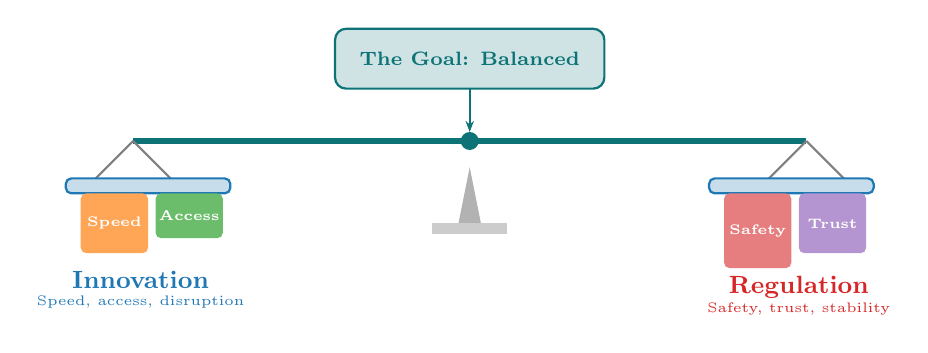
\begin{tikzpicture}[scale=0.95]

  % ---- Fulcrum and beam -----------------------------------
  % Fulcrum triangle
  \fill[mlgray!60] (-0.15,-1.6) -- (0.15,-1.6) -- (0,-0.85) -- cycle;
  \fill[mlgray!40] (-0.5,-1.75) rectangle (0.5,-1.6);

  % Main beam
  \draw[mlteal,line width=2.5pt] (-4.5,-0.5) -- (4.5,-0.5);
  \fill[mlteal] (0,-0.5) circle (0.12);

  % ---- Left pan: Innovation --------------------------------
  % Pan strings
  \draw[mlgray,thick] (-4.5,-0.5) -- (-3.8,-1.2);
  \draw[mlgray,thick] (-4.5,-0.5) -- (-5.2,-1.2);
  % Pan dish
  \fill[mlblue!25,draw=mlblue,thick,rounded corners=2pt]
    (-5.4,-1.2) rectangle (-3.2,-1.0);
  % Items on left pan (innovation)
  \fill[mlorange!70,rounded corners=2pt] (-5.2,-2.0) rectangle (-4.3,-1.2);
  \node[font=\tiny\bfseries,text=white,align=center] at (-4.75,-1.6) {Speed};
  \fill[mlgreen!70,rounded corners=2pt] (-4.2,-1.8) rectangle (-3.3,-1.2);
  \node[font=\tiny\bfseries,text=white,align=center] at (-3.75,-1.5) {Access};
  % Label
  \node[font=\small\bfseries,text=mlblue] at (-4.4,-2.35) {Innovation};
  \node[font=\tiny,text=mlblue] at (-4.4,-2.65) {Speed, access, disruption};

  % ---- Right pan: Regulation (heavier -- tilted beam shows tension) -----
  \draw[mlgray,thick] (4.5,-0.5) -- (3.8,-1.2);
  \draw[mlgray,thick] (4.5,-0.5) -- (5.2,-1.2);
  \fill[mlblue!25,draw=mlblue,thick,rounded corners=2pt]
    (3.2,-1.2) rectangle (5.4,-1.0);
  % Items on right pan (regulation)
  \fill[mlred!60,rounded corners=2pt]   (3.4,-2.2) rectangle (4.3,-1.2);
  \node[font=\tiny\bfseries,text=white,align=center] at (3.85,-1.7) {Safety};
  \fill[mlpurple!70,rounded corners=2pt] (4.4,-2.0) rectangle (5.3,-1.2);
  \node[font=\tiny\bfseries,text=white,align=center] at (4.85,-1.6) {Trust};
  % Label
  \node[font=\small\bfseries,text=mlred] at (4.4,-2.45) {Regulation};
  \node[font=\tiny,text=mlred] at (4.4,-2.75) {Safety, trust, stability};

  % ---- Sweet spot annotation --------------------------------
  \fill[mlteal!20,rounded corners=4pt] (-1.8,0.2) rectangle (1.8,1.0);
  \draw[mlteal,thick,rounded corners=4pt] (-1.8,0.2) rectangle (1.8,1.0);
  \node[font=\scriptsize\bfseries,text=mlteal] at (0,0.6) {The Goal: Balanced};

  % Arrow down to fulcrum
  \draw[mlteal,-{Stealth[length=4pt]},thick] (0,0.2) -- (0,-0.38);

\end{tikzpicture}
\end{center}
\vspace{-0.3em}
\begin{block}{}
\scriptsize
\textbf{The governance question:}
``Innovation without consumer protection is risk transfer from institutions to individuals.''\\
This course gives you the frameworks to evaluate \emph{both sides of the scale}.
\end{block}
\bottomnote{Each lecture in this course adds evidence. By L07 you will be able to place any fintech innovation on this scale and defend the placement.}
\end{frame}

% ============================================================
%  FRAME 10 -- ACT: Activity frame (5-question evaluation framework)
% ============================================================
\begin{frame}{Act: Evaluate Any Fintech in Five Questions}

\vspace{0.2em}
\begin{columns}[T]
\begin{column}{0.56\textwidth}
\begin{block}{The Fintech Evaluation Framework}
\small
\begin{enumerate}
  \item \textbf{Who is the customer?}\\
        {\scriptsize Consumer, SME, enterprise, or another fintech?}
  \vspace{3pt}
  \item \textbf{What value-chain layer does it attack?}\\
        {\scriptsize Origination, distribution, servicing, or infrastructure?}
  \vspace{3pt}
  \item \textbf{How does it make money?}\\
        {\scriptsize Fees, subscription, data monetisation, or interest float?}
  \vspace{3pt}
  \item \textbf{What is its regulatory position?}\\
        {\scriptsize Licensed, white-labelled, or operating in a gap?}
  \vspace{3pt}
  \item \textbf{Does it create or capture value?}\\
        {\scriptsize New markets (inclusion) or share from incumbents?}
\end{enumerate}
\end{block}
\end{column}
\begin{column}{0.40\textwidth}
\vspace{0.4em}
\begin{exampleblock}{Try It Now}
\scriptsize
Pick \textbf{one} financial app on your phone.\\[4pt]
Work through the five questions.\\[4pt]
Is the app from a:\\[-2pt]
\begin{itemize}\scriptsize
  \item Traditional bank?
  \item Fintech startup?
  \item Big tech platform?
\end{itemize}
\vspace{4pt}
What does your answer reveal about the \textbf{collaboration model} in use?
\end{exampleblock}
\vspace{0.5em}
\begin{alertblock}{Next Lecture}
\scriptsize \textbf{L02 -- Fintech Ecosystem}\\
Growth drivers, financial inclusion, trust, and behavioural dimensions.\\
\textit{11:30 today -- bring your app count!}
\end{alertblock}
\end{column}
\end{columns}

\bottomnote{These five questions work for any fintech -- in the news, in a VC pitch, or in your career. You will use this framework in the Workshop C evaluation exercise on Day 5.}
\end{frame}

% ============================================================
\end{document}
% ============================================================
